\chapter{Introduction\label{cha:intro}}
\epigraph{Learning is not a product of schooling, but the lifelong attempt to
acquire it}{\textit{Albert Einstein}}
\noindent
The concept of lifelong learning has become very popular over the last decade.
The original idea has gone through a lot of changes, through the stages of
continuing, recurrent, and adult education \citep{Jarvis2004}. On one hand, the
lifelong learning concept has an entirely economic background, where the
learners themselves are seen as tools for economic development and their needs
are firmly tied to the needs of the industry (Carter, 2008, pp. 112-114). On the
other hand, as stated by UNESCO, \LLLs is a cultural policy which influences
society and promotes changes (Boshier, 2000, pp. 12- 14). However, no matter
which point of view is adopted, world economics, employment policy and society
are changing. The importance of lifelong learning is increasing. For full
participation in education, workplace, and society individuals today require
well-developed lifelong learning skills, developed from the early stages of
their lives (Otala, 1997).

In addition to being a subject for political and economical discussions
\citep{Bagnall2009}, \LLLs has been also established as a topic of interest in
higher education, in particular universities \citep{Knapper2000}. Based on this
background of the importance of lifelong learning and the central role of
universities, this research project is focused on and explores the need for
lifelong learning support in universities.

In addition to being a subject for political and economical discussions
\citep{Bagnall2009}, \LLLs has been also established as a topic of interest in
higher education, in particular universities \citep{Knapper2000}. Based on this
background of the importance of lifelong learning and the central role of
universities, this research project is focused on and explores the need for
lifelong learning support in universities.

In addition to being a subject for political and economical discussions
\citep{Bagnall2009}, \LLLs has been also established as a topic of interest in
higher education, in particular universities \citep{Knapper2000}. Based on this
background of the importance of lifelong learning and the central role of
universities, this research project is focused on and explores the need for
lifelong learning support in universities.

\section{Reseach Goals}

The overall aim of this research is to design and implement a learner-centered e-learning
environment which will support and facilitate the lifelong learning process in universities.
This environment will be built on an institutionally focused Learning Management
System and a learner focused ePortfolio system, both already used in universities. A
review of this field showed that these two areas are already connected, but to adequately
support lifelong learning they need to better meet the requirements of both students and
education providers (universities) as lifelong learning stakeholders.

\section{Research Design}

The overall aim of this research is to design and implement a learner-centered e-learning
environment which will support and facilitate the lifelong learning process in universities.
This environment will be built on an institutionally focused Learning Management
System and a learner focused ePortfolio system, both already used in universities. A
review of this field showed that these two areas are already connected, but to adequately
support lifelong learning they need to better meet the requirements of both students and
education providers (universities) as lifelong learning stakeholders.

\section{Scope and Limitations}

This research project has its limitations. Although technology is usually called
a key driver in the educational change \citep{Attwell2007}, one can argue that
it is not only a technical question \citep{Schaffert2008}. Many other changes
should occur to fully implement lifelong learning in universities: changes in
the way of thinking of both students and lecturers, support on the higher
(department or institutional) levels, provision of technical support and
trainings for staff, personal motivation of learners, etc. As technology is one
of the components of fully supported lifelong learning environment, this project
is focused on technical aspects. The other aspects will stay behind the focus of
this research, but state of the art, literature and theories in the area have
been still comprehensively investigated.

\section{Thesis Structure and Outline}

The rest of this thesis is structures as follows:

\begin{figure}[htb]
\centering
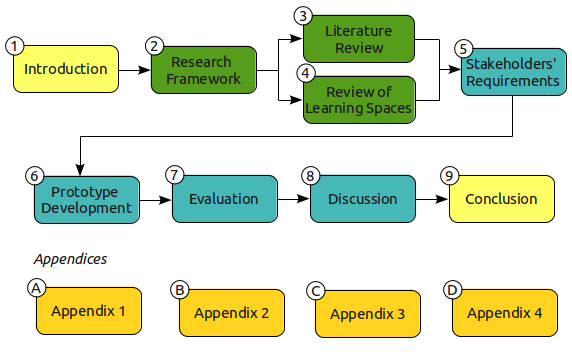
\includegraphics[width=0.8\textwidth]{CH1-F1-Thesis}
\caption{Thesis structure}
\label{fig:ts}
\end{figure}

\begin{description}
\item[Chapter 2.] This chapter presents a menthodological approach employed in
this reseach. Theoretical background of design science research methodology is
given and the way this appoach was adopted in this project is described.
\item[Chapter 3.] This chapter focused on discussing the background of \LLLsn.
Its connection to universities, the current situation in this area and the
problems associated with \LLLs in universities are shown here.
\item[Chapter 4.] This chapter explores the technical worlds of learning
support. System that are curently mployed at universities are examined according
to their compliance with \LLLs support.
\item[Chapter 5.] The results of literature review (Chapter 3) and a review of
learning spaces (Chapter 4) are taken to the stakeholders for analysis of their
needs and requirements. Later these findings are used in developemnt of a conceptual model
of an environment that can provide support for \LLLsn.
\item[Chapter 6.] Implementation process and outcomes are presented in this
chapter.
\item[Chapter 7.] This chapter describes a complex evaluation design used in the
research to address the questions of quality, functionality and suitability of
the developed features.
\item[Chapter 8.] In this chapter the results and lessons learnt are discussed.
\item[Chapter 9.] This chapter brings conclusion of the research presented in
this thesis and implications for future research.
\end{description}